\section{Infrared Radiation Transfer Material}\label{infrared-radiation-transfer-material}

One of the important technical features of EnergyPlus is that the fundamental zone model includes infrared (IR) radiation exchange among all surfaces within the zone. A zone can consist of a single room or multiple rooms having similar thermal characteristics. The other fundamental characteristic of a zone in EnergyPlus is that the air within the zone is modeled with the assumption that it is well-stirred, so it is characterized by a single uniform air temperature. Normally, this corresponds to the desired physical state of the air within a zone. Practically, this is accomplished with the mixing caused by the air distribution system or even with the addition of ceiling fans. However, there are situations where the well-stirred model condition does not fit the physical conditions within a space (e.g., large atria spaces, displacement ventilation systems, and under floor air distribution systems). In these cases, the air temperature varies spatially within the zone, but the surfaces in the regions that have different air temperatures still exchange IR radiation with the other surfaces in the zone, even those in regions having a different air temperature.

Historically, several approaches have been taken to model such situations. They all involve unrealistically modifying the convective heat transfer characteristics within a single zone to produce reasonable total heat transfer for the zone while maintaining the zone IR radiation in its basic form. The IRT model takes a different, more fundamental approach. The space is divided into subzones, each having the basic well-stirred air model, but surfaces in these subzones are able to exchange IR radiation with other surfaces throughout the original space. Any convective air exchange between subzones is handled using the existing flexible capabilities within EnergyPlus. In other words, the subzones are standard EnergyPlus zones but they have been given the capability of allowing IR radiation to be exchanged with surfaces in adjacent zones.

The IR radiation exchange is accomplished by introducing special IR Transparent (IRT) surfaces to link adjacent zones. These surfaces transmit the IR radiation incident on them to the surfaces in adjacent zone. The special surfaces have no thermal resistance, and they also have zero convective heat transfer coefficients on both sides. Consider a stratified atrium as an example. The atrium would be divided into stacked vertical zones, with each zone having the special IRT surface between it and the next lower zone. All physical surfaces in the two zones exchange radiation with the IRT surface, but it does not impede the transfer of radiation from one zone to the other. On each side it interacts as a black body surface and any radiation incident on it is absorbed. Since it has no other heat transfer mechanisms, it comes to equilibrium with zero net radiation transfer.

Schematic diagrams of the application of the IRT surfaces are shown in Figure~\ref{fig:schematic-view-of-stacked-zones} and Figure~\ref{fig:schematic-model-of-a-ufad-zone}. The first figure shows it applied between two stacked zones that could be part of an atrium. All radiation incident on the IRT in the lower and upper zone is completely absorbed by the surface. It is prevented from participating in the zone air heat balance by fixing the heat transfer coefficients on either side at zero.

\begin{figure}[hbtp] % fig 20
\centering
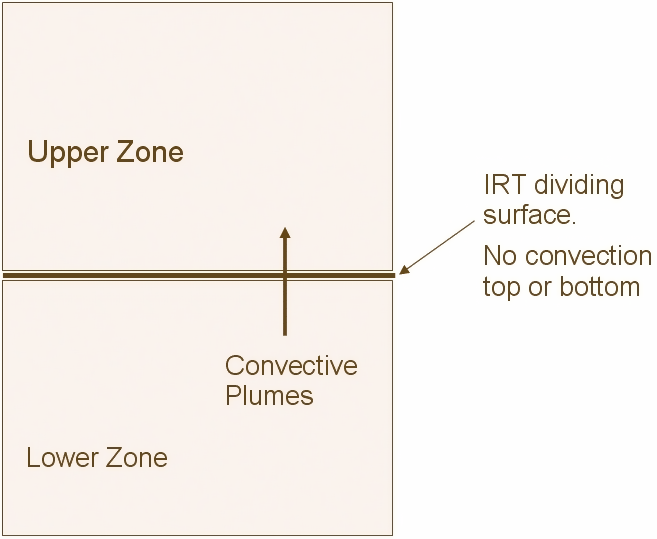
\includegraphics[width=0.9\textwidth, height=0.9\textheight, keepaspectratio=true]{media/image390.png}
\caption{Schematic View of Stacked Zones \protect \label{fig:schematic-view-of-stacked-zones}}
\end{figure}

The same arrangement can be used for simulating a underfloor air distribution system (UFAD). The two zones represent the lower occupied (mixed) zone and the upper stratified zone. Since the upper zone is being modeled as a mixed EnergyPlus zone, it is not precisely the stratified zone concept. However, if a user has concern about having the entire upper part of the space at a single average temperature, the space could be modeled with two stacked upper zones. In that case the stratified temperature profile would be established by the relative size of the mixing from the convective plumes. The user would have to supply those estimates from external knowledge of the behavior of UFAD systems and plumes.

\begin{figure}[hbtp] % fig 21
\centering
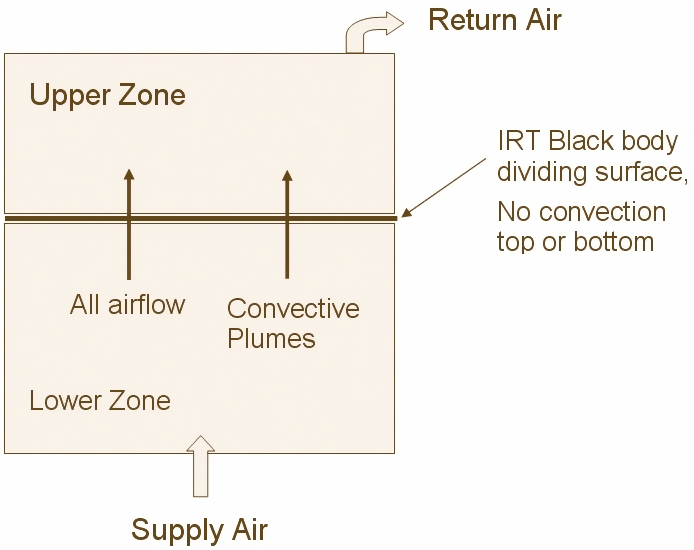
\includegraphics[width=0.9\textwidth, height=0.9\textheight, keepaspectratio=true]{media/image391.png}
\caption{Schematic Model of a UFAD Zone \protect \label{fig:schematic-model-of-a-ufad-zone}}
\end{figure}

\subsection{Radiation Exchange Basics}\label{radiation-exchange-basics}

The behavior of the IRT surface can be analyzed by considering three parallel black plates infinite in extent, as shown in Figure~\ref{fig:radiation-exchange-model}. The outside plates are held at two different temperatures, and the intermediate plate assumes an equilibrium temperature when the net heat flux goes to zero. All plates have black body surface characteristics.

\begin{figure}[hbtp] % fig 22
\centering
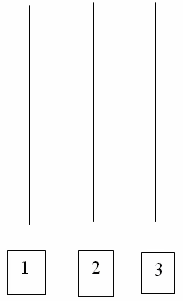
\includegraphics[width=0.9\textwidth, height=0.9\textheight, keepaspectratio=true]{media/image392.png}
\caption{Radiation Exchange Model \protect \label{fig:radiation-exchange-model}}
\end{figure}

The radiant exchange between surface 1 and 2 is:

\begin{equation}
{q_{1 - 2}} = \sigma A\left( {T_1^4 - T_2^4} \right)
\end{equation}

The exchange between surfaces 2 and 3 is:

\begin{equation}
{q_{2 - 3}} = \sigma A\left( {T_2^4 - T_3^4} \right)
\end{equation}

Equating heat fluxes and eliminating T\(_{2}\) gives:

\begin{equation}
{q_{1 - 3}} = \frac{\sigma }{2}A\left( {T_1^4 - T_3^4} \right)
\end{equation}

where:

q is the heat flux in W/m\(^{2}\)

$\sigma$ is the Stephan Boltzman constant

A is the plate area in m\(^{2}\), and

T is the temperature in K.

Equation shows that the presence of a black body surface between a source and a sink reduces the heat flux by a factor of two. The same result occurs when the IRT surface is between two zones in EnergyPlus. In that case the adjacent zones behave as black body cavities at some equivalent temperature. In order to account for this reduction, the IRT area must be doubled. This can be done without any difficulty in the EnergyPlus radiant exchange routine because the radiation view factors are determined by an approximate procedure that is based on the areas of the surfaces. Thus, doubling the surface area of the IRT surface results in the correct transfer of radiation through the IRT surface. The doubling will occur automatically in the program as described in the Input Output Reference document.

It should be noted that, because of the black body behavior of the IRT surface, any visible or solar short wavelength radiation incident on the surface will be absorbed and included with the long wavelength (IR) exchange with the adjacent zone. No energy will be lost, but zones with IRT surfaces should not be used in any lighting analyses.

\subsection{Radiation Transfer Surface Details}\label{radiation-transfer-surface-details}

\subsubsection{Specifying an Infrared Transparent (IRT) surface}\label{specifying-an-infrared-transparent-irt-surface}

The Infrared Transparent (IRT) surface is similar to a resistance-only surface. The idd object for this type of surface is shown below. The fields indicate that the surface will actually participate in the transfer of visible and solar radiation by doing a wavelength transformation and making all short wavelength radiation that is incident on the surface into long wavelength radiation and having it participate in the long wavelength radiant exchange. The Material:InfraredTransparent object requires only a name. All other parameters are set internally.

The Infrared Transparent surface should not participate in a convective/conductive exchange between the zones it separates. In order to minimize this effect, the SurfaceProperty:ConvectionCoefficients object must be used. Outside and Inside values for the surface's convection coefficients should be on the order of .1.~ Further examples are given in the Input Output Reference document.

\subsection{Behavior Checks}\label{behavior-checks}

The behavior of multi zones separated with infrared transparent surfaces can be checked with a simple comparison. Begin with a single zone model as shown below. This model has a south-facing window, and four walls exposed to wind and sun, and a roof exposed to wind and sun.

\begin{figure}[hbtp] % fig 23
\centering
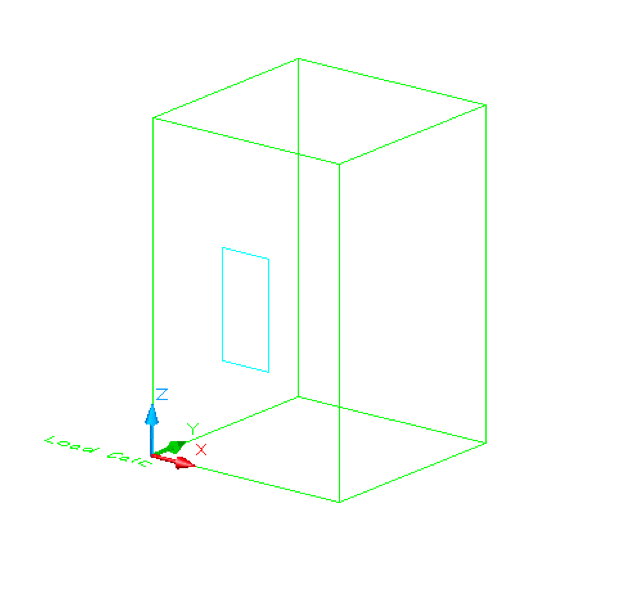
\includegraphics[width=0.9\textwidth, height=0.9\textheight, keepaspectratio=true]{media/image396.png}
\caption{Single Zone Model \protect \label{fig:single-zone-model}}
\end{figure}

The single zone model will be compared with a stacked three zone model that has zones separated by interzone infrared transparent surfaces. This model is shown below.

\begin{figure}[hbtp] % fig 24
\centering
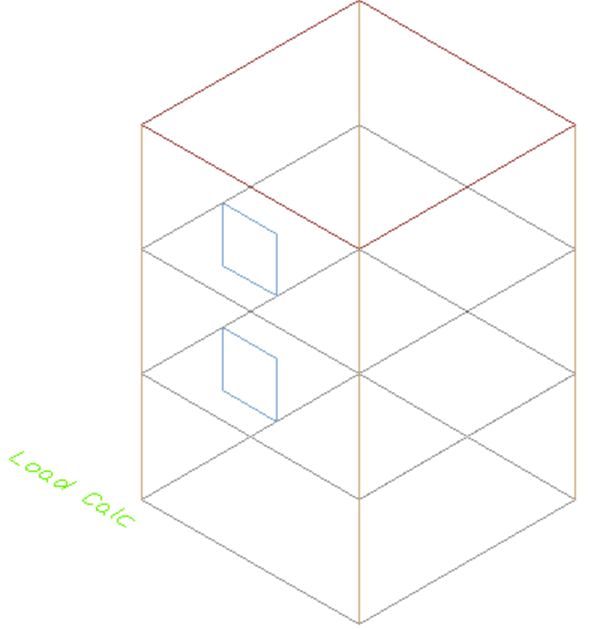
\includegraphics[width=0.9\textwidth, height=0.9\textheight, keepaspectratio=true]{media/image397.png}
\caption{Stacked Three Zone Model \protect \label{fig:stacked-three-zone-model}}
\end{figure}

The two upper zones have south facing windows whose total area is the same as the area of the single window in the single zone model. The top and the sides are again exposed to sun and wind. The separating surfaces are modeled as IRT surfaces. All zones in both models are controlled at the same setpoint temperature using purchased air.

The sensible heating results are shown below. The results show the sum of the sensible cooling load for the three stacked zones and the single zone. It is clear that the IRT surfaces are very effective in transmitting infrared radiation between the zones. Some small differences, such as those shown, will occur because of the conversion from short wavelength solar to infrared through the special IRT dividing surfaces.

\begin{figure}[hbtp] % fig 25
\centering
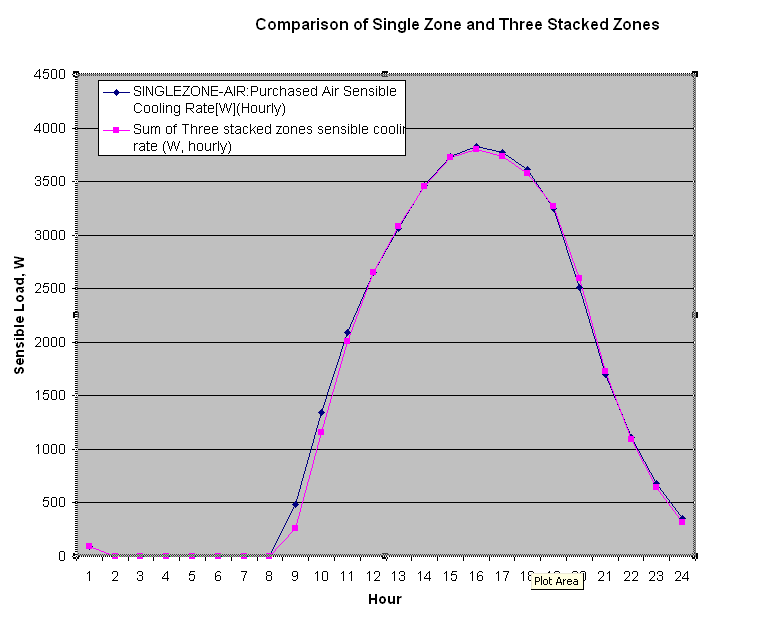
\includegraphics[width=0.9\textwidth, height=0.9\textheight, keepaspectratio=true]{media/image398.png}
\caption{Comparison of Single and Three Stacked Zones \protect \label{fig:comparison-of-single-and-three-stacked-zones}}
\end{figure}
